\section{Development of the Calibration Source}

\subsection{Tritiated Methane Removal}
\label{sec:RD}

The removal efficiency of zirconium getters for methane in xenon had previously been studied at the University of Maryland.  It was found that greater than 99.99\% of natural methane can be removed in a single pass through a zirconium getter. \cite{Dobi_CH4} Tritiated methane is chemically identical to natural methane, so it follows that similar removal efficiencies should be expected for CH$_3$T.  To verify this a small scale tritiated methane injection system was integrated into a liquid xenon system at the University of Maryland.  This system used a SAES MC1-905F methane purifier placed in series immediately after the CH$_3$T source bottle to prevent non-methane species of tritium from entering the plumbing. Over 68,000 Bq of observed CH$_3$T activity was injected into this small scale system and a removal efficiency of over 99.99\% for tritiated methane in xenon was confirmed.

\begin{figure}[h!]\centering
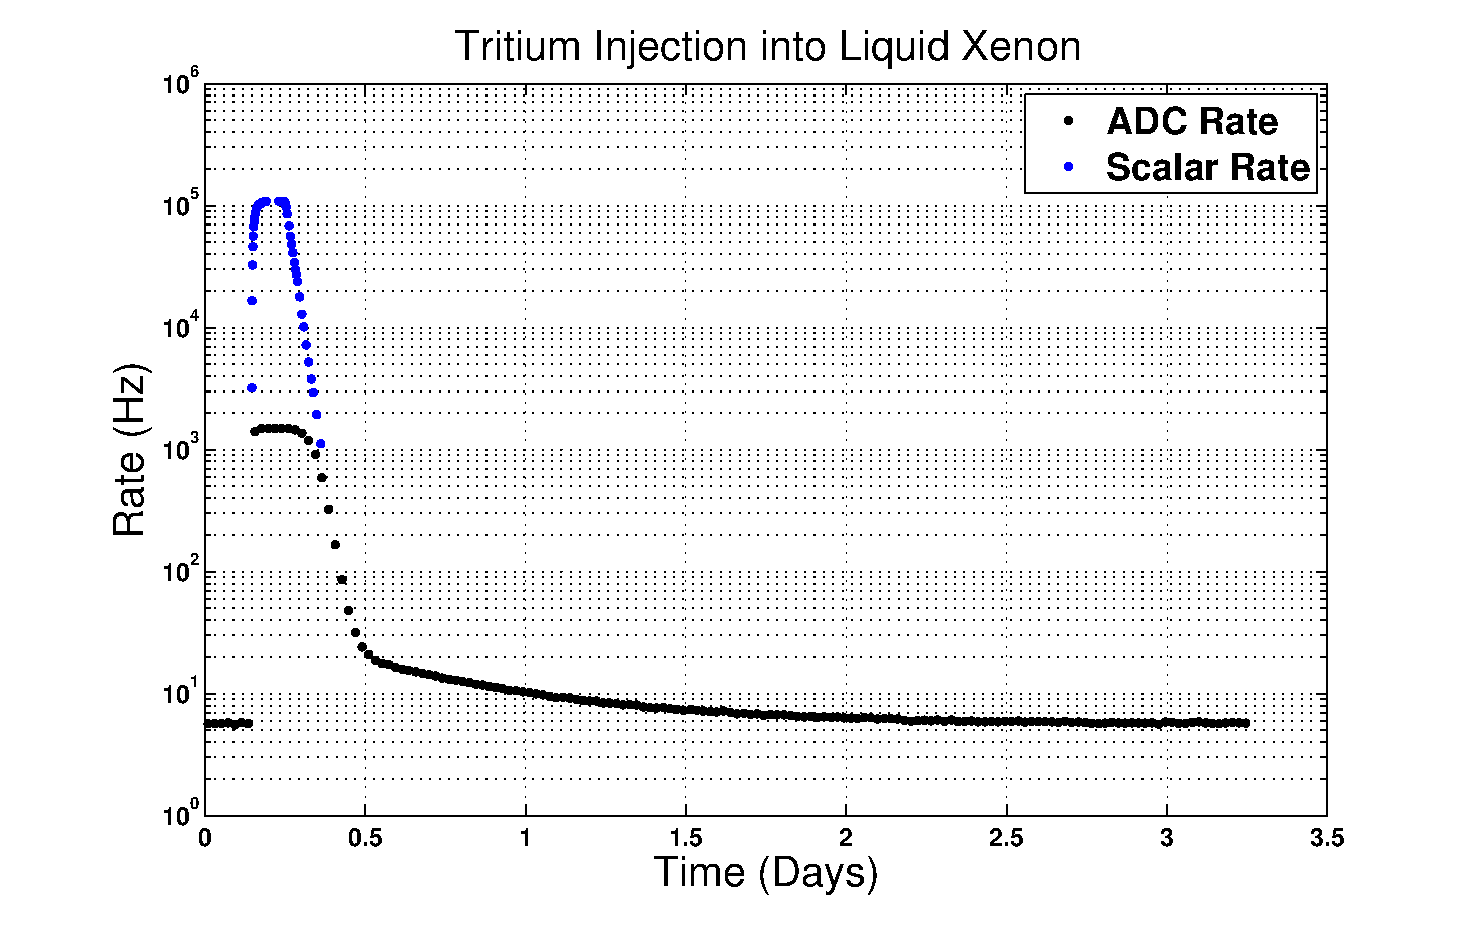
\includegraphics[width=80mm]{TimeHisto_Analog2.eps}
\caption{A time histogram of the event rate during a tritium injection into our small scale detector. The event rate greatly exceeded the limits of our ADC (black data points), so a analog scalar was used to count the true event rate (blue data points). }
\label{fig:Density}
\end{figure}


\subsection{Out Gassing of Tritiated Methane from Plastics}

\newcommand*{\Scale}[2][4]{\scalebox{#1}{$#2$}}%

An accurate model of a tritiated methane injection into LUX must account for out gassing of CH$_3$T from plastics such as polyethylene and teflon.  Using data from the liquid xenon experiments at the University of Maryland we numerically modeled the purification and residual diffusion of CH$_3$T in the detector.  Using Duhamel's priciple, the analytic solution to Fick's second law on a half-infite line is
\[\Scale[0.5]{\phi (x,t) = KC_{out} - \int \limits_0^t erf(\frac{x}{\sqrt{4D(t - \tau)}})K\dot{C_{out}}(\tau)d\tau - KC_{out}(0)erf(\frac{x}{\sqrt{4Dt}}),}\]
where $K$ is the solubility of the material, $D$ is the diffusion constant, and $C_{out}$ is the outside concentration of the material. 
%\cite{Piche}
For the out gassing process we are only able to detect the flux of material out of the plastic.  This is given by Fick's first law evaluated at $x=0$,
\[J_{out}(t)= - K \sqrt{\frac{D}{\pi}}( \int \limits_0^t \frac{\dot{C_{out}}(\tau)}{\sqrt{t-\tau}} d \tau + \frac{C_{out}(t)}{\sqrt{t}}),\]
where the sign has been flipped since the flux of material is outward.  We see that it is no longer possible to evaluate $K$ and $D$ separately, since the diffusion in and out of the plastic is completely determined by the time-dependent concentration outside of the plastic.  To simplify our model, we define a new constant
\[ G = K \sqrt{ \frac{D}{ \pi }} .\]
By fitting the integral of the flux out of the plastic over time to out gassing data collected in Maryland's liquid xenon system we constrain $G \leq 0.01 \; \frac{cm}{\sqrt{day}}.$ 

With a constraint on $G$ taken from the analytic solution to Fick's second law, we turn to numerical simulation to answer the question of how much initial CH$_3$T activity to inject into LUX to meet our calibration conditions.  Several assumptions are made to simplify the numerical model.  First, we approximate the diffusion into plastic as being a one dimensional process.  Since the plastic in our detector at Maryland and in LUX can be approximated by a cylindrical shell, there is no dependence on the azimuthal or $z$ coordinates.  Since $r$ is large compared to the thickness of the plastic shell, $\frac{\delta^2 \phi}{\delta r^2} \gg \frac{1}{r} \frac {\delta \phi}{\delta r}$, so Fick's laws in a one dimensional approximation become
\[J=-D\frac{\delta \phi}{\delta r}\vec{r}\]
\[\frac{\delta \phi}{\delta t} = D \frac{\delta^2 \phi}{\delta r^2}.\]  We assume the concentration of CH$_3$T in LUX is uniform throughout its volume, since the design of LUX creates currents which stir the liquid xenon.  With perfect mixing the effect of the purifier can be modeled by adding an exponential time dependence to the outer volume.  The time constant of this decay has an upper limit equal to the time it takes xenon to recirculate through the LUX detector, although in reality the mass transport from diffusion in the liquid and gaseous xenon decreases this time constant. 

We use a simple implementation of the first order Euler method for our numerical simulations. The diffusion is simulated by setting the concentration at the boundary of the piece equal to $KC_{out}$, where $C_{out}$ is the concentration of CH$_3$T in the xenon.  This concentration is dependent on time according to
\[\frac{\delta C_{out}}{\delta t} = J_{out} \frac{A_{plastic}}{V_{xenon}}-\frac{C_{out}}{\tau},\]
where $A_{plastic}$ is the surface area of the plastic cylinder, $V_{xenon}$ is the total volume of xenon in the fiducial region, and $\tau$ is the time it takes for one full purification cycle.  The first term on the right of this equation models out gassing of CH$_3$T from the plastic cylinder, while the second term models removal of CH$_3$T through purification.  Using the first order Euler method, we arrive at an expression for $C_{out}$ given by
\[C_{j+1}=C_j + \Delta t [(J_{1,j}-J_{N_x,j})\frac{A_{plastic}}{V_{xenon}}-\frac{C_j}{\tau}].\]
The initial concentration is defined by dividing the desired injection activity by the volume of the fiducial region.  We choose $D = 2.3 \times 10^{-9} \frac {cm^2}{sec}$ so that the half-infinite boundary conditions in our diffusion model is valid, and combine this with our allowed range of values for $G$ to extract a value for $K$.  We use this model to predict the total number of calibration events as well as the time required to return to \textless 5\% of the nominal background rate for any CH$_3$T injection into LUX.  

\begin{figure}[h]
\centering
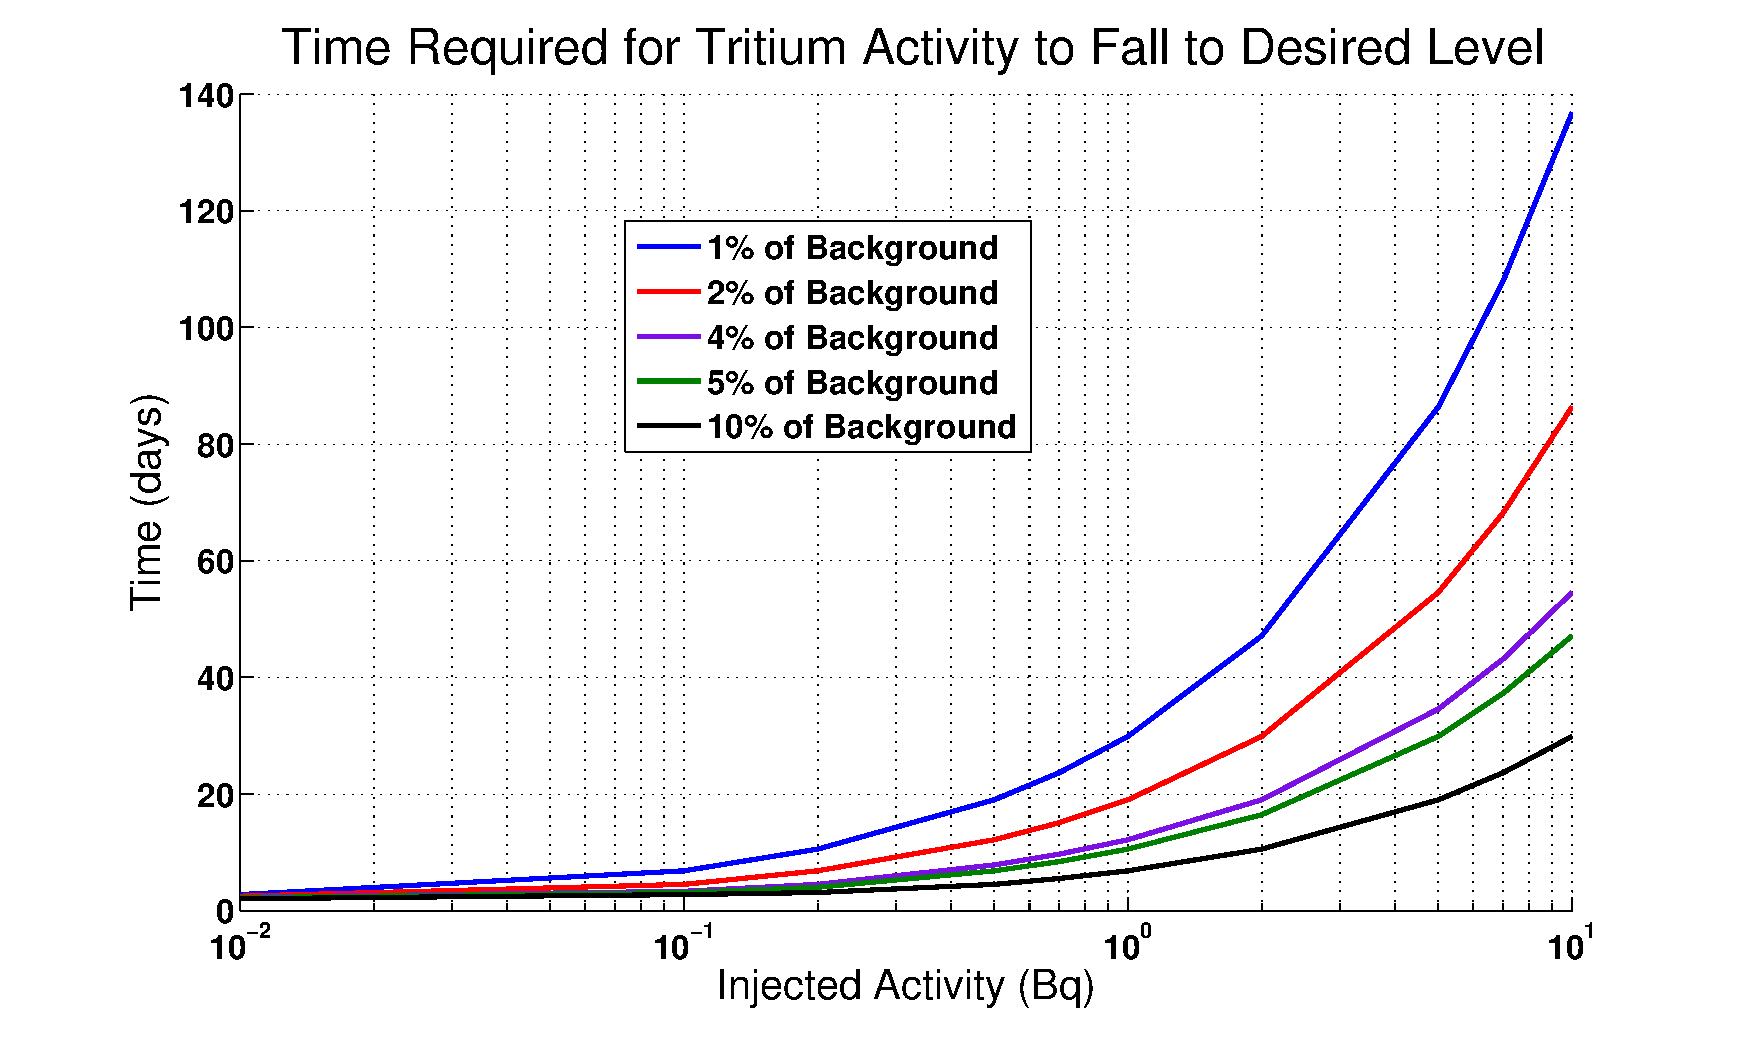
\includegraphics[scale=0.25]{LUXfig_INJvar_time_new.eps}
\caption{Time required to remove CH$_3$T from LUX after various injections.}
\label{fig:CH3TREMOVAL}
\end{figure}


\section{Implementation of the Calibration Source}

\subsection{Injection System Hardware}

The setup of our triated methane calibration technique can be separated into three parts: the tritiated methane source bottle, the injection system,  and the zirconium getter.

The tritiated methane source bottle for our calibration technique consists of a 2250 cc stainless steel bottle which is filled with a mixture of tritiated methane and purified xenon.  The purpose of this xenon is to serve as a carrier gas for the tritiated methane.  The total activity in the source bottle is set by mixing tritiated methane from a reservoir into the source bottle via volume sharing.

The injection system for our tritiated methane calibration technique consists of a series of expansion volumes which are used to fine tune the amount of CH$_3$T that is injected.  Once the CH$_3$T source bottle is opened it flows through a methane gas purifier (SAES MC1-905F) to remove any non-methane species of tritium, such as bare tritium. The expansion volumes are then filled with tritiated methane from the source bottle, and the flow of xenon in the gas system is diverted through the expansion volumes to sweep the CH$_3$T into the detector downstream of the LUX xenon purifier.  A pump out port allows the expansion volumes to be evacuated in preparation for each use of the injection system.  

The LUX gas system uses a hot zirconium getter (SAES-PS4MT15R1) located upstream of the CH$_3$T injection system to remove CH$_3$T from the xenon after passing through the detector.  

\begin{figure}[H]\centering
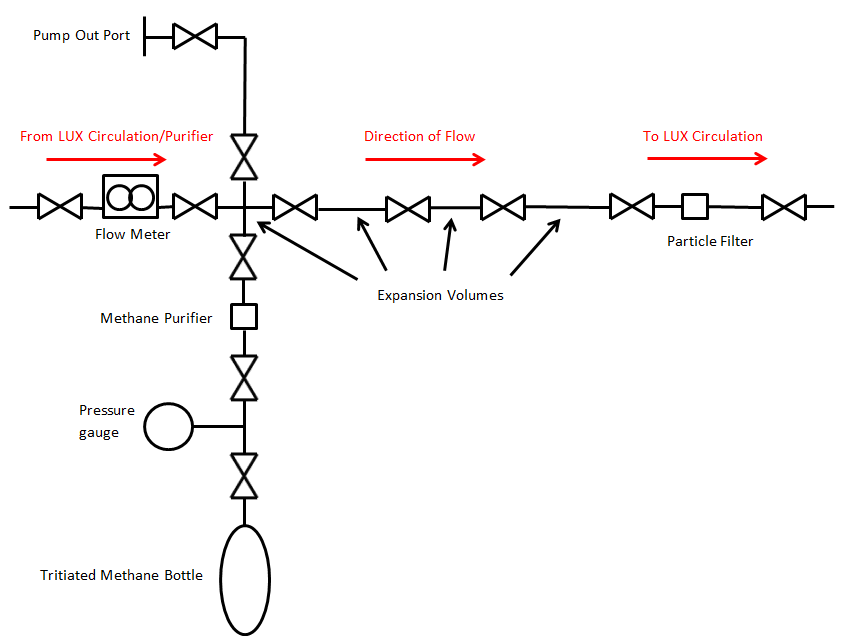
\includegraphics[width=80mm]{TritiumPlumbing.png}
\caption{Plumbing diagram of the tritium injection system for LUX.  Tritium is injected downstream of the LUX xenon purifier so that it passes through the detector once prior to being removed.  Red arrows indicate the direction of flow.}
\label{fig:Removal}
\end{figure}

\subsection{Natural Methane Injection}


Figure ?? shows that a large purification time constant can lead to long wait times before the residual tritiated methane rate returns to acceptable levels. To measure the purification time constant in LUX 0.02 grams of natural methane were injected into LUX prior to injecting tritiated methane.  Purity samples from the detector were collected over the next few days, and a purification time constant of 5.90 $\pm$ 0.07 hours was determined using data collected with the LUX gas sampling system. The measured time constant was much smaller than expected based on xenon circulation rates alone, allowing for a larger injection of tritiated methane into the detector.  


(INSERT JON'S PURIFICATION TIME CONSTANT PLOT)

\begin{figure}[h!]\centering
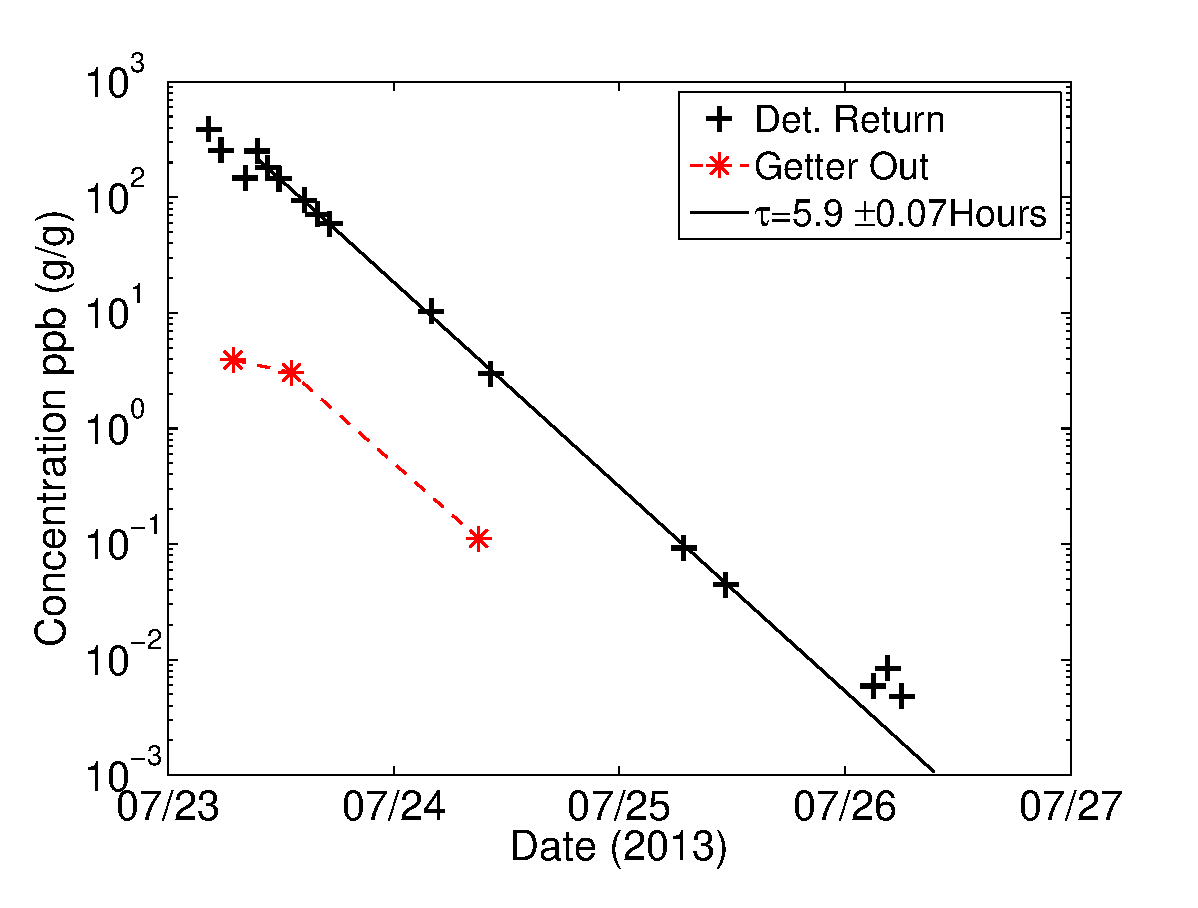
\includegraphics[width=80mm]{CH4_injection_3.eps}
\caption{Removal of natural methane observed by the integrated xenon sampling system prior to the tritiated methane injections. The red points indicate xenon gas measurements at the getter outlet, we find a 97\% one pass removal efficiency at a flow rate of 25 SLPM. 1 $\rm 10^{-3}$ ppb (g/g) is the limit of detection for methane using the LUX gas sampling system.}
\label{fig:Removal_methane}
\end{figure}


\begin{comment} %% AD
\subsection{Tritiated Methane Injection}

To confirm the purification model established by the natural methane injection a small amount of tritiated methane was injected into LUX the following week. An absolute activity of 20 mBq of tritiated methane was injected with the getter in purify mode.  Thus as soon as the CH3T passed through the detector it was immediately removed.  A purification time constant of 6.7 hours was observed, consistent with the natural methane purification rate measured by the sampling system. After a day of circulating through the getter the tritium decay had fallen below detectable amounts confirming the effective removal of the tritiated methane with the getter. 

After confirming our purification model a larger injection of 800 mBq was performed. This second injection produced 20,000 beta decay events in the LUX detector before being completely removed, 5000 of those events could be used the calibrate the ER band in the WIMP search region of 0-30 Phe (pulse area in photo electrons). 
Figure \ref{fig:Removal} shows the two tritium injections and the subsequent CH3T purification. The rate of tritiated methane removal was consistent with the previous two injections $\rm 1/10^5$.


\begin{figure}[h!]\centering
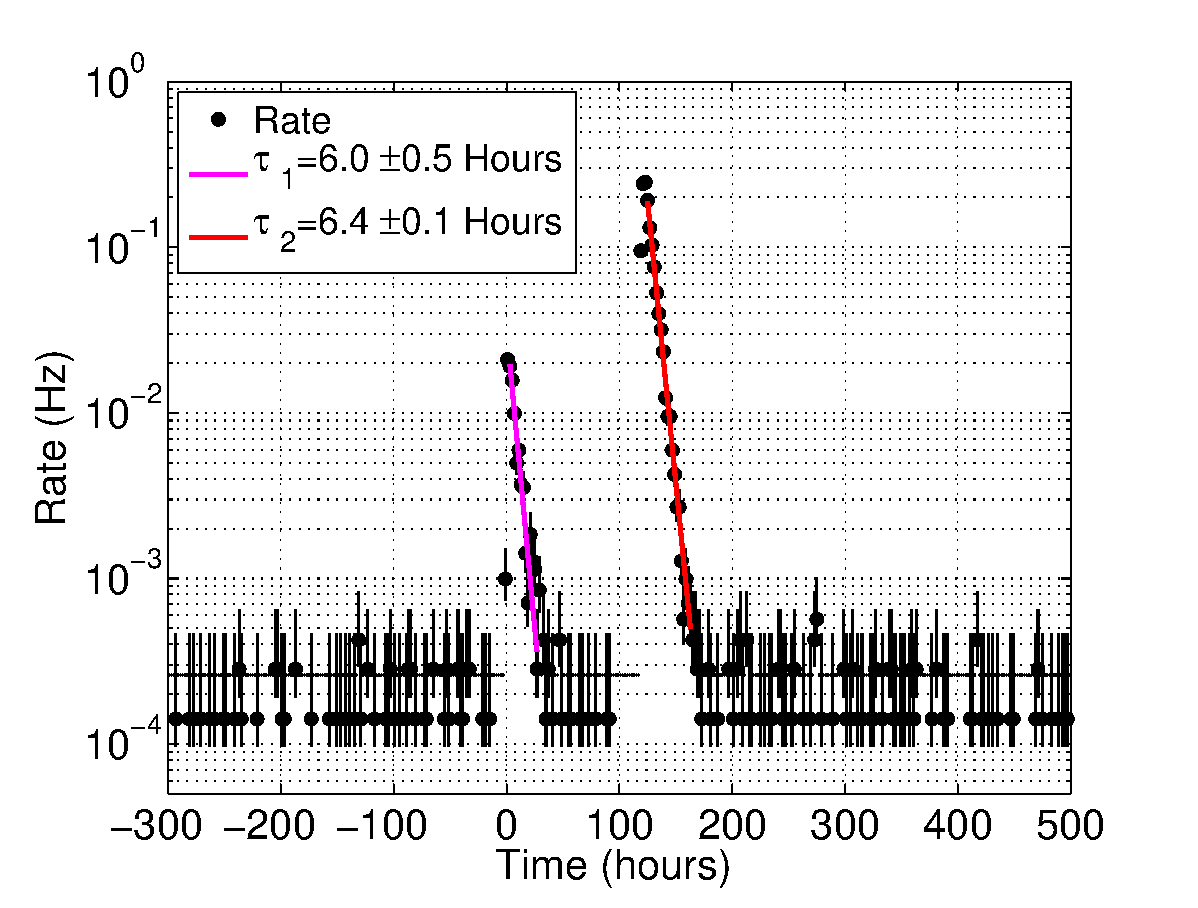
\includegraphics[width=80mm]{CH3T_Rate_fid_150_Run03_Tritium_Rate.eps}
%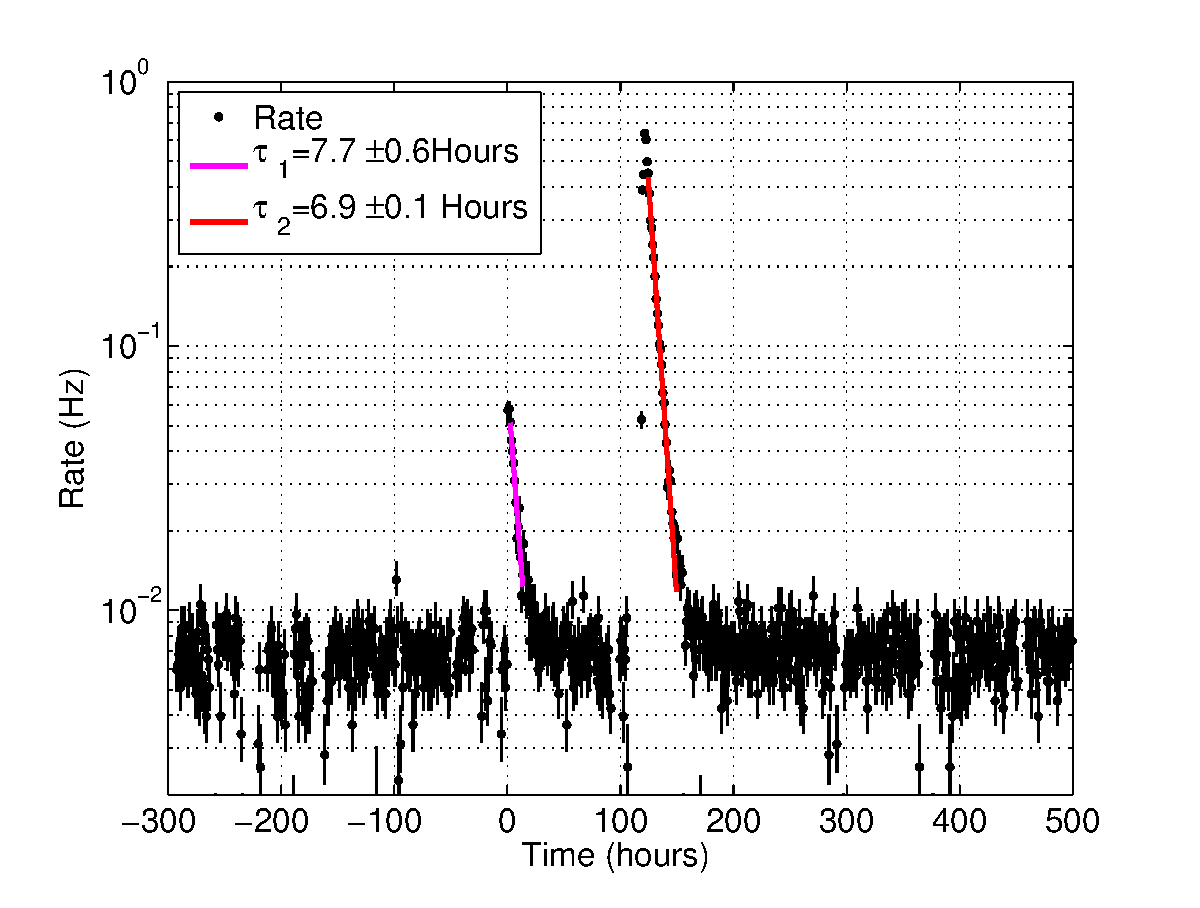
\includegraphics[width=60mm]{CH3T_Rate_Nofid_150_Run03_Tritium_Rate}
\caption{Rate of single scatter events with S1 below 150 Phe in the fiducial volume. 150 Phe in S1 is about 18.6 $\rm keV{ee}$, the endpoint to the tritium beta spectrum. The magenta and red curves are fits to the first and second tritium injection's removal rate.}
\label{fig:Removal}
\end{figure}

\end{comment}%% AD